\begin{figure}[h!]
	\centering
	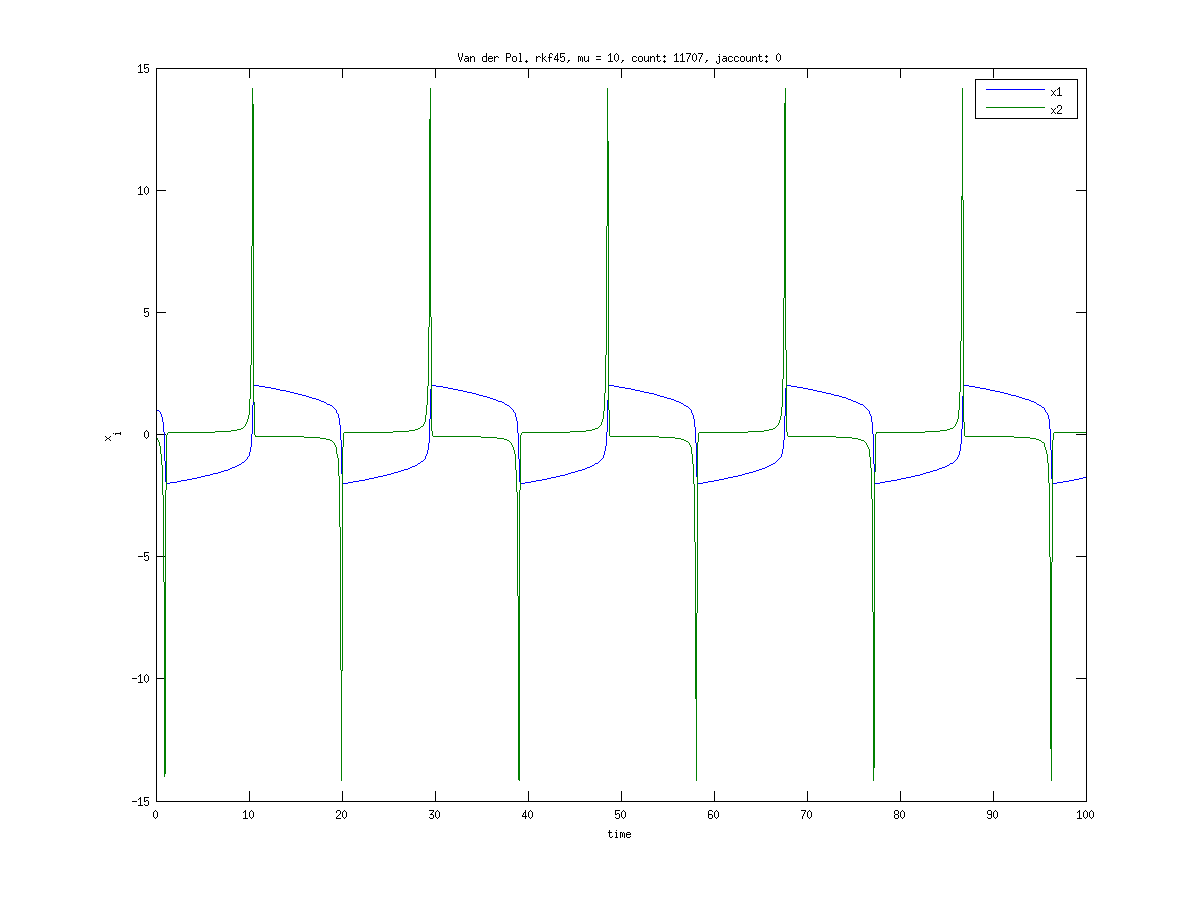
\includegraphics[width=0.8\textwidth]{img/exc1_45_10}
	\caption{Van der Pol model. Solved using rkf45 with parameter $\mu = 10$.}
	\label{fig:exc1_45_10}
\end{figure}

\begin{figure}[h!]
	\centering
	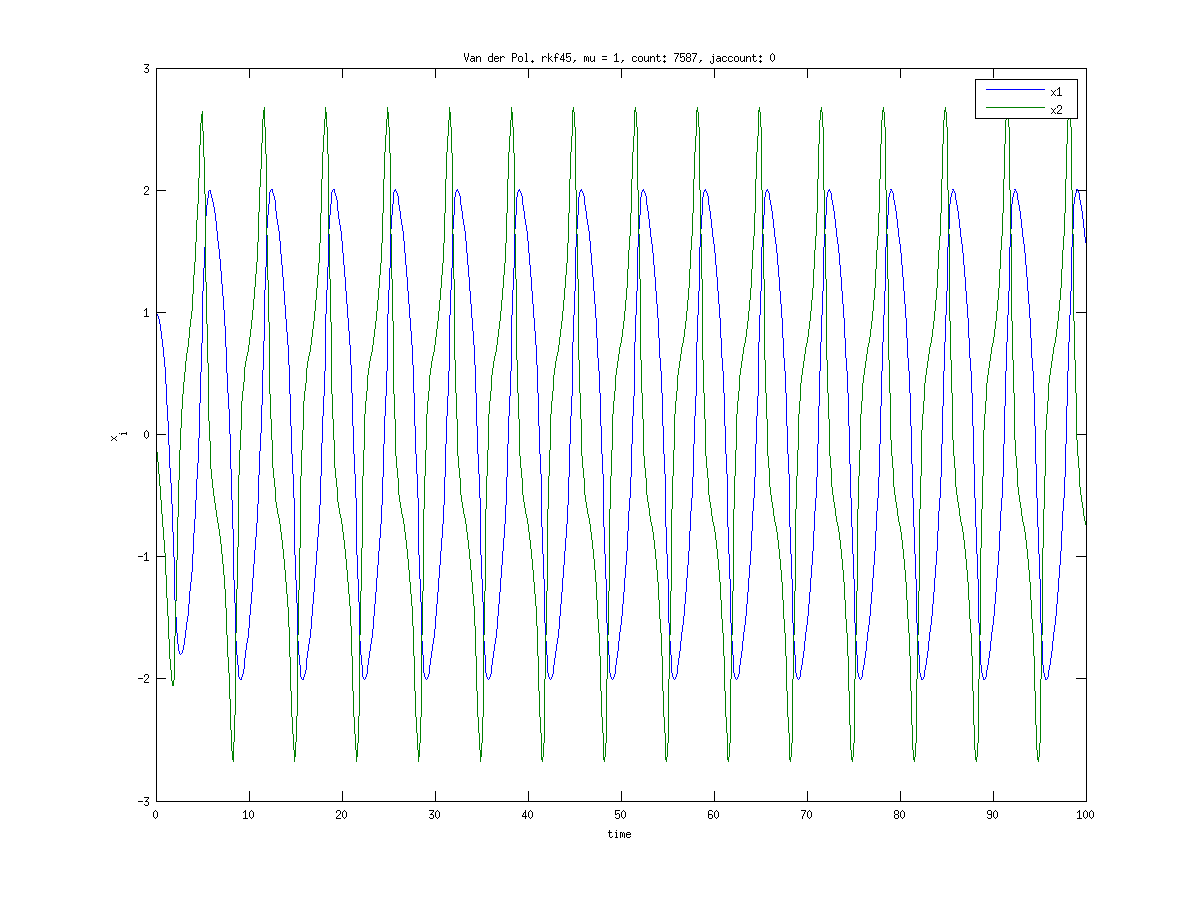
\includegraphics[width=0.8\textwidth]{img/exc1_45_1}
	\caption{Van der Pol model. Solved using rkf45 with parameter $\mu = 1$.}
	\label{fig:exc1_45_1}
\end{figure}

\begin{figure}[h!]
	\centering
	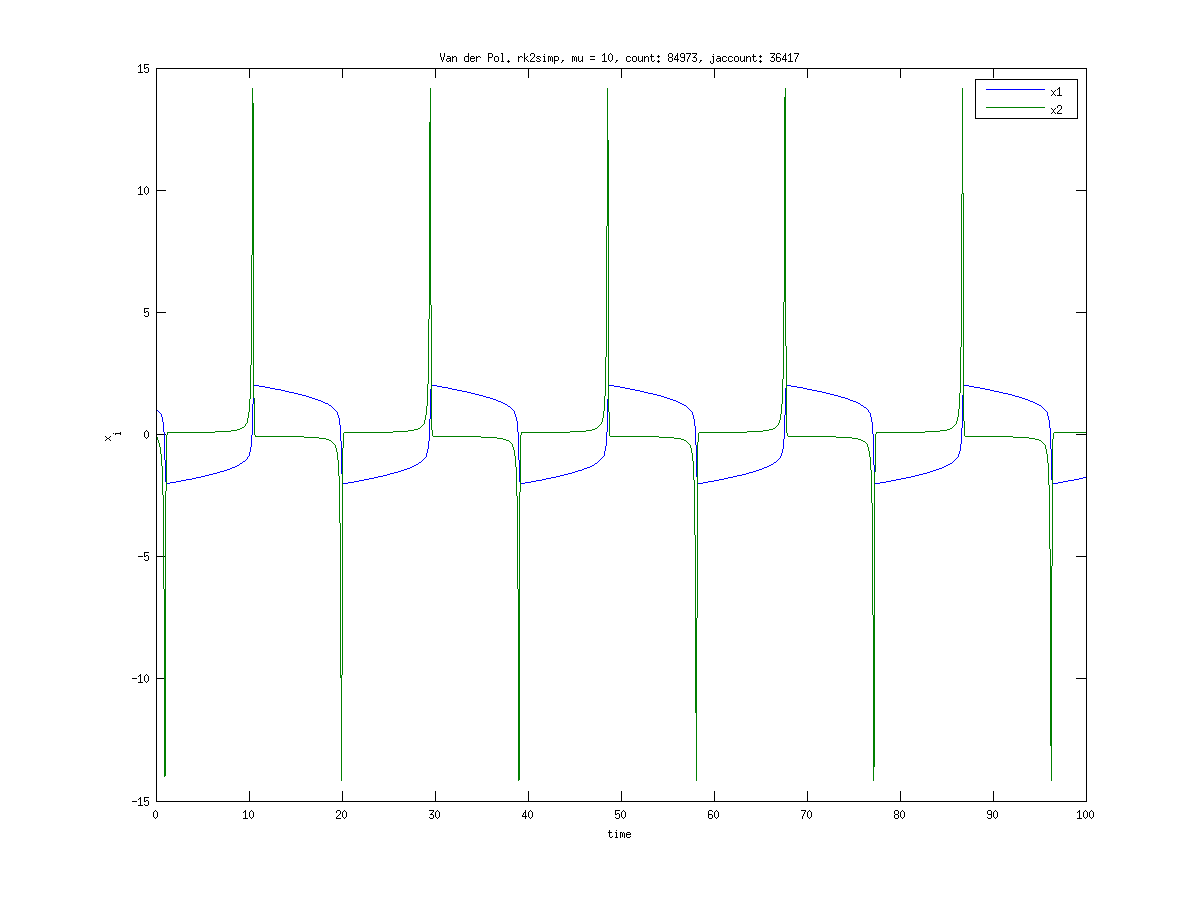
\includegraphics[width=0.8\textwidth]{img/exc1_2_10}
	\caption{Van der Pol model. Solved using rk2simp with parameter $\mu = 10$.}
	\label{fig:exc1_2_10}
\end{figure}

\begin{figure}[h!]
	\centering
	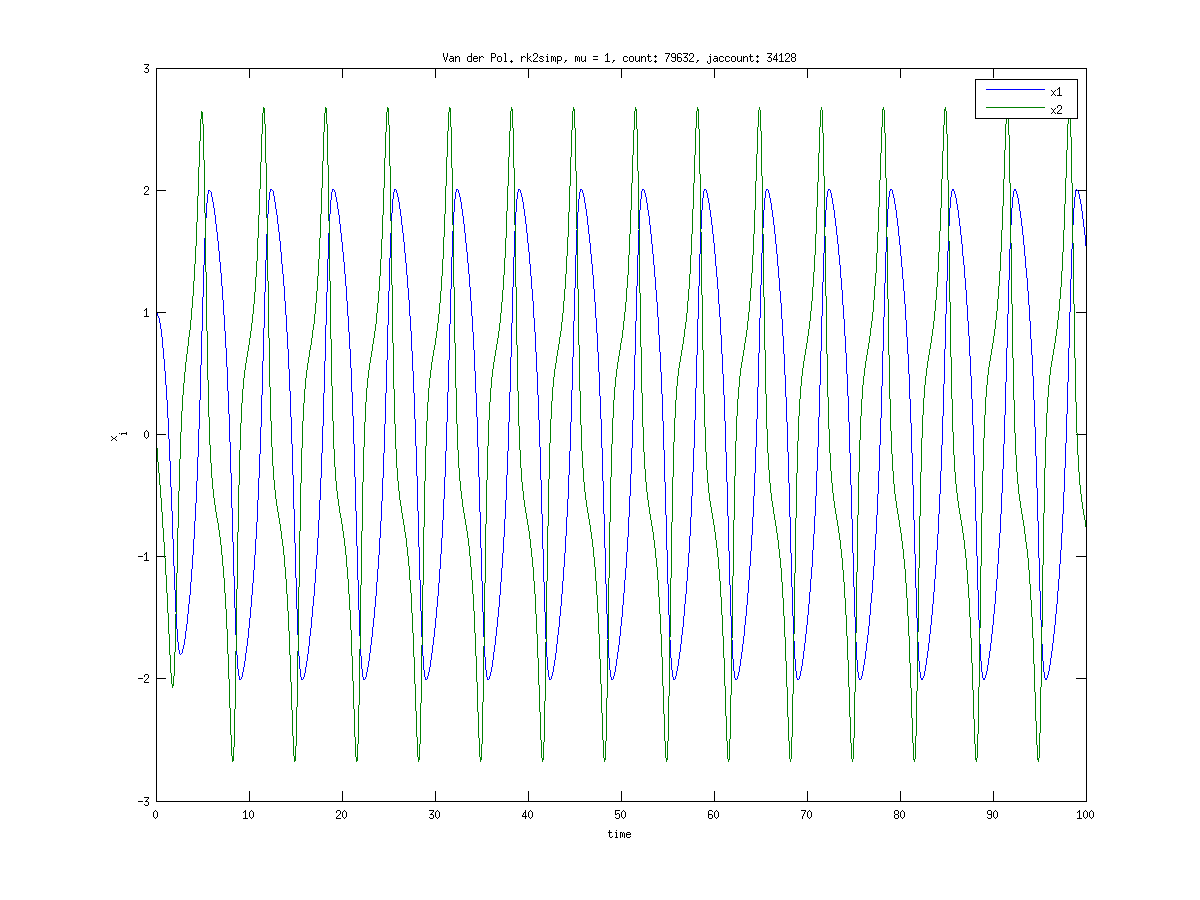
\includegraphics[width=0.8\textwidth]{img/exc1_2_1}
	\caption{Van der Pol model. Solved using rk2simp with parameter $\mu = 1$.}
	\label{fig:exc1_2_1}
\end{figure}